\documentclass[11pt,aspectratio=169]{beamer}

\usepackage[utf8]{inputenc}
\usepackage[T1]{fontenc}
\usepackage[ngerman]{babel}
\usepackage{graphicx}
\usepackage{etoolbox}
\usepackage{tabu}

\usetheme{Montpellier}

\title{Workshop: Smarthomesensoren mit Home Assistant}
\author{Marian Ulbricht}
\date{\today}
\newcommand{\presenter}{marian.ulbricht@htwk-leipzig.de}

\usepackage{style/mypresi}
\setbeamercovered{transparent}

\begin{document}

\begin{frame}
  \maketitle
\end{frame}

\begin{frame}{Inhalt}
  \tableofcontents
\end{frame}

\section{Motivation}

\begin{frame}{Was haben wir heute vor~\ldots}
  \begin{itemize}
    \item Wir bauen ein \textit{Smart-Home-System} mit einer Steuerzentrale,
      einem Sensor und einem Aktor.
    \item Wir benutzen dafür nur Komponenten, die quelloffen sind und bei denen
      wir verstehen können, was im Hintergrund passiert (also nichts von Apple
      oder Microsoft).
  \end{itemize}

  \begin{block}{Zielstellung}
    Sie bekommen heute eine ausführliche Anleitung zum Zusammenbau eines kleinen
    Smart-Home-Systems, das Sie auch leicht zu Hause nachbauen können. Alle
    notwendigen Schritte können mit diesem PDF und dem Repository unter
    \url{https://github.com/ulbricht-inr/hassio_esp_sensorworkshop}
    nachvollzogen werden.
  \end{block}
\end{frame}

\section{Hardware}

\begin{frame}{Hardware, die wir benutzen I}
  \begin{block}{Raspberry Pi}
    \begin{itemize}
      \item Mini-Computer mit mehreren Kernen und genug Rechenleistung, um als
        Office-PC genutzt zu werden. Als Betriebssystem kommt Linux zum Einsatz.
      \item Gebaut als Lehr- und Lernplattform, mit Zugang zu
        Hardware-Komponenten wie GPIO, ADC und Feldbussen.
      \item Besitzt eine sehr große Online-Community mit vielen Anleitungen und
        Hilfestellungen. \textbf{Jeder Schüler sollte einen haben!}
    \end{itemize}
    \centering
    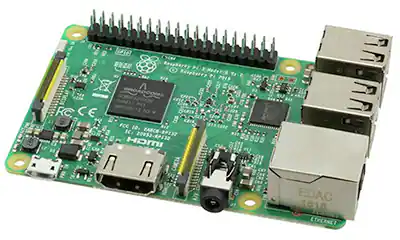
\includegraphics[width=0.25\textwidth]{bilder/rpi.png}
  \end{block}
\end{frame}

\begin{frame}{Hardware, die wir benutzen II}
  \begin{block}{ESP8266}
    \begin{itemize}
      \item Mikrocontroller mit WLAN.
      \item Kann sehr viel für einen kleinen Preis und besitzt ähnliche
        Schnittstellen wie der Raspberry Pi.
      \item Die Programmierung ist kompliziert. Daher nutzen wir heute eine
        Vereinfachung, um aus einer Textdatei ein komplettes Betriebssystem zu
        bauen.
    \end{itemize}
    \centering
    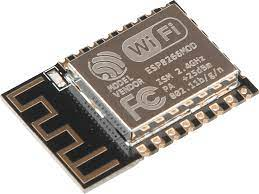
\includegraphics[width=0.25\textwidth]{bilder/esp.jpeg}
  \end{block}
\end{frame}

\begin{frame}{Hardware, die wir benutzen III}
  \begin{block}{DHT11}
    \begin{itemize}
      \item Temperatur- und Luftfeuchtigkeitssensor.
      \item Braucht nur eine Datenleitung zur Kommunikation.
    \end{itemize}
    \centering
    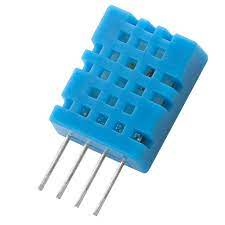
\includegraphics[width=0.25\textwidth]{bilder/dht11.jpeg}
  \end{block}
\end{frame}

\begin{frame}{Hardware, die wir benutzen IV}
  \begin{block}{LED}
    \begin{itemize}
      \item Halbleiterbauelement, das Licht aussendet.
    \end{itemize}
    \centering
    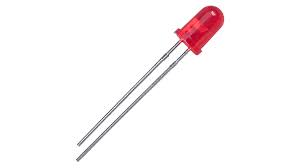
\includegraphics[width=0.36\textwidth]{bilder/led.jpeg}
  \end{block}
\end{frame}

\section{Software}

\begin{frame}{Software, die wir benutzen I}
  \begin{block}{Home Assistant}
    \begin{itemize}
      \item In der Programmiersprache Python geschriebene
        Automatisierungssoftware.
      \item Leicht erweiterbar, Open Source und kostenlos.
      \item Unterstützt eine sehr große Anzahl unterschiedlicher Komponenten
        von unterschiedlichen Herstellern.
      \item \url{https://www.home-assistant.io/}
    \end{itemize}
    \centering
    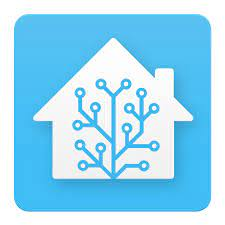
\includegraphics[width=0.20\textwidth]{bilder/ha.jpeg}
  \end{block}
\end{frame}

\begin{frame}{Software, die wir benutzen II}
  \begin{block}{ESPHome}
    \begin{itemize}
      \item Hilfssoftware, die aus einer kleinen Textdatei ein ganzes
        Betriebssystem für den ESP8266 erzeugt.
      \item \url{https://esphome.io/}
    \end{itemize}
    \centering
    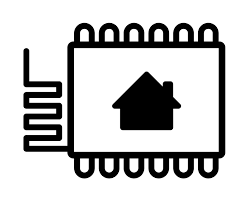
\includegraphics[width=0.20\textwidth]{bilder/esphome.png}
  \end{block}
\end{frame}

\end{document}
